\chapter{Экспериментальная часть}
\label{cha:research}

В данной части будет проведена апробация и тестирование разработанной программы.

\section{Примеры работы}

% примеры со скриншотами интерфейса
Программа имеет консольный интерфейс. Далее будут приведены скриншоты.

\begin{figure}
    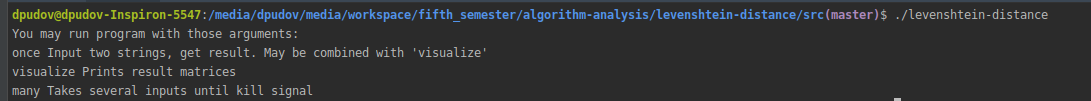
\includegraphics[width=0.9\textwidth]{screenshots/screenshot-usage}
    \caption{Использование программы.}
    \label{screenshot-usage}
\end{figure}

\begin{figure}
    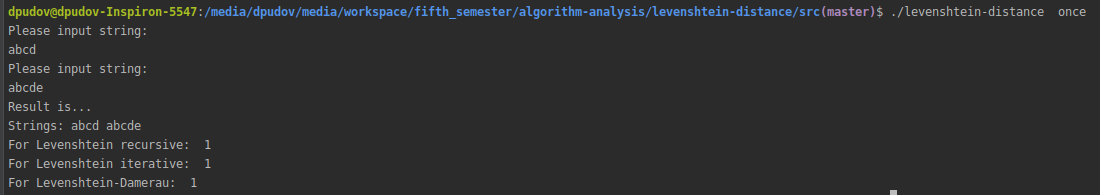
\includegraphics[width=0.9\textwidth]{screenshots/screenshot-once}
    \caption{Однократное использование.}
    \label{screenshot-once}
\end{figure}

\begin{figure}
    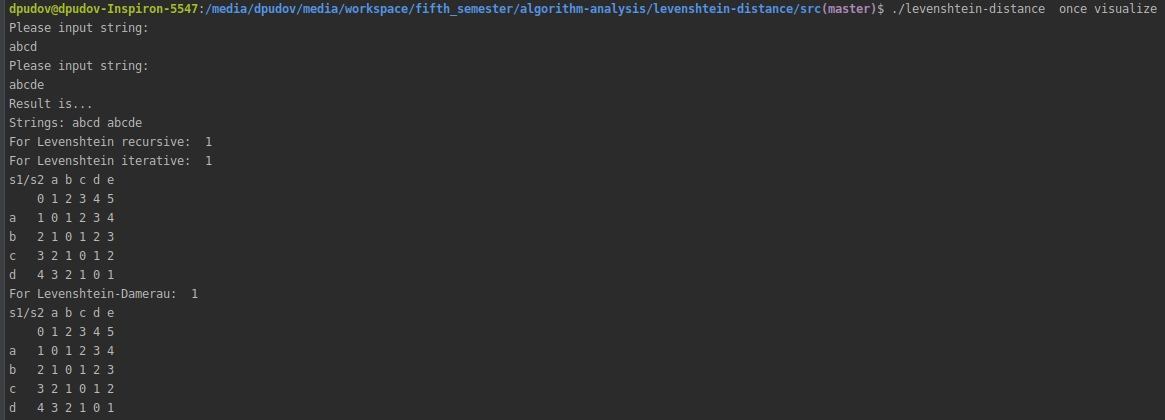
\includegraphics[width=0.9\textwidth]{screenshots/screenshot-visualize}
    \caption{Использование с выводом матриц.}
    \label{screenshot-visualize}
\end{figure}

\begin{figure}
    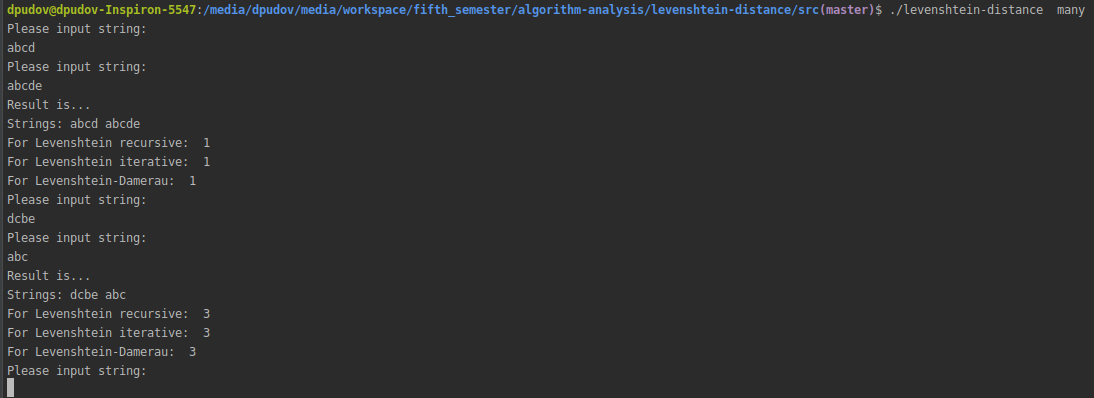
\includegraphics[width=0.9\textwidth]{screenshots/screenshot-many}
    \caption{Многократное использование.}
    \label{screenshot-many}
\end{figure}

\FloatBarrier

\section{Результаты тестирования}

\section{Постановка эксперимента по замеру времени и памяти}

\section{Сравнительный анализ на материале экспериментальных\\ данных}

% Эксперименты + выводы
